\chapter{Cowlitz County, Washington}
\label{ch:cowlitz_county}

As this is the first linguistic analysis of the speech in Cowlitz County, I felt that a brief description of the area was requisite because it is necessary to understand the context in which these linguistic changes are embedded. I will briefly describe the area's geography since the abundance of trees and proximity to rivers ultimately played an important role in the growth of the timber industry there. What then follows is a brief history of the region, including the Cowlitz people, the settlement of the first people of European descent, colonization, Longview and the Long-Bell Company and the demographic shift that ensued, and the rise and fall of the mills during the 20th Century.

This chapter draws heavily from four sources. The first is a small book entitled \textit{Cowlitz County Washington 1854 - 1948} written by Hattie Barlow Olson\footnote{Her name as it appears on the book is Mrs. Charles H. Olsen but \citet[177]{urrutia_1998} mentions her by name.} and published by the Kelso Chamber of Commerce in 1948. Olson's parents were some of the original founders of Kelso and she relates several first-hand accounts of the early days of Cowlitz County. The second work is \textit{They Came to Six Rivers: The Story of Cowlitz County} by Virginia Urrutia, published by the Cowlitz County Historical Society in 1998. Urrutia is also a descendent of some of the original founders of the area and a long-time editor of the \textit{Cowlitz Quarterly}. Another is \textit{R. A. Long's Planned City: The Story of Longview} by John M. McClelland, Jr., published by the Longview Publishing Co. in 1976. McClelland is the son of the first editor of the local paper, the \textit{Longview Daily News}. The last is \textit{Whistles: The Story of Longview Fibre Company} by David Wilma, a historian with family ties to the area, who personally interviewed many longtime residents.\footnote{I am grateful to David Wilma and also to Bill Watson of the Cowlitz Historical Museum for sharing with me the audio to many of these interviews and many other recordings of lifelong Cowlitz County residents. I acquired them too late for them to be incorporated into this dissertation, but they will provide an invaluable source for tracking language change in real time in southwest Washington. } A few details from my own interviews are sprinkled throughout where relevant.

\section{A physical description of Cowlitz County}
\label{sec:physical_description}

\begin{figure*}[p]
    \centering
    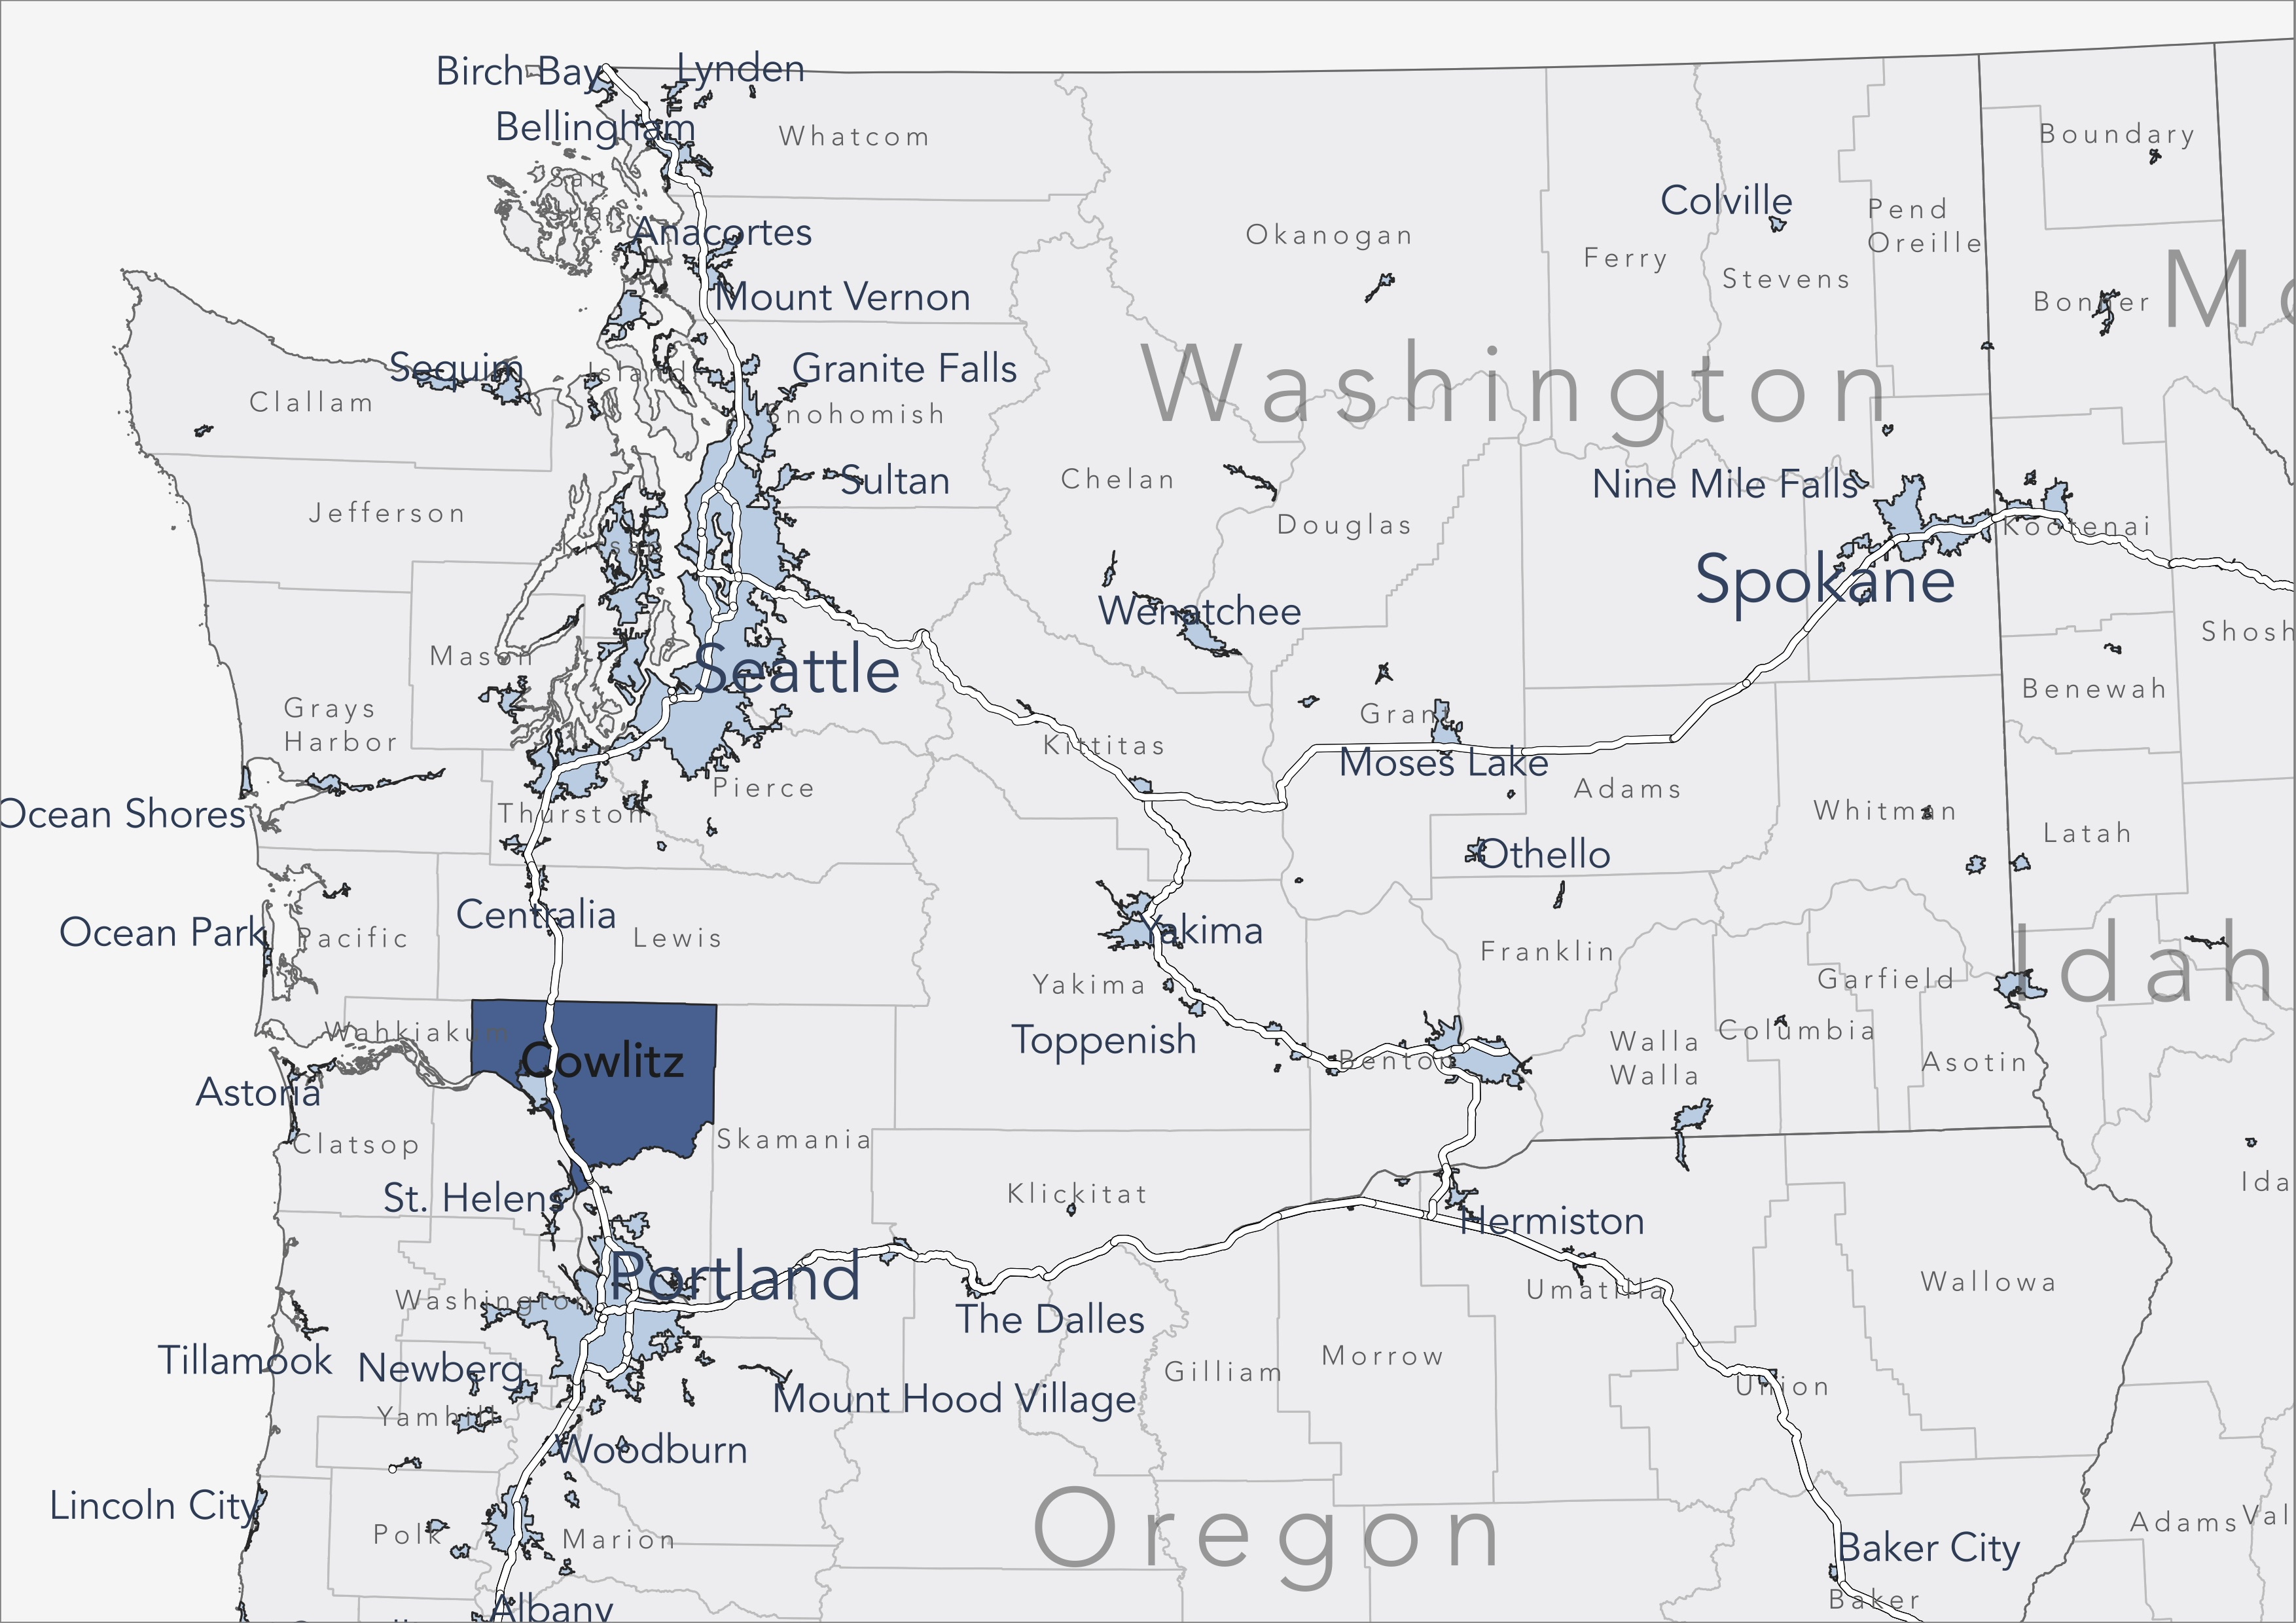
\includegraphics[angle=90, origin=c, width = 5.75in]{Figures/other_figures/Cowlitz_Context_small.jpg}
    \caption{Cowlitz County, Washington and its position in the Pacific Northwest}
    \label{fig:map_of_cowlitz_big}
\end{figure*}

\begin{figure*}[p]
    \centering
    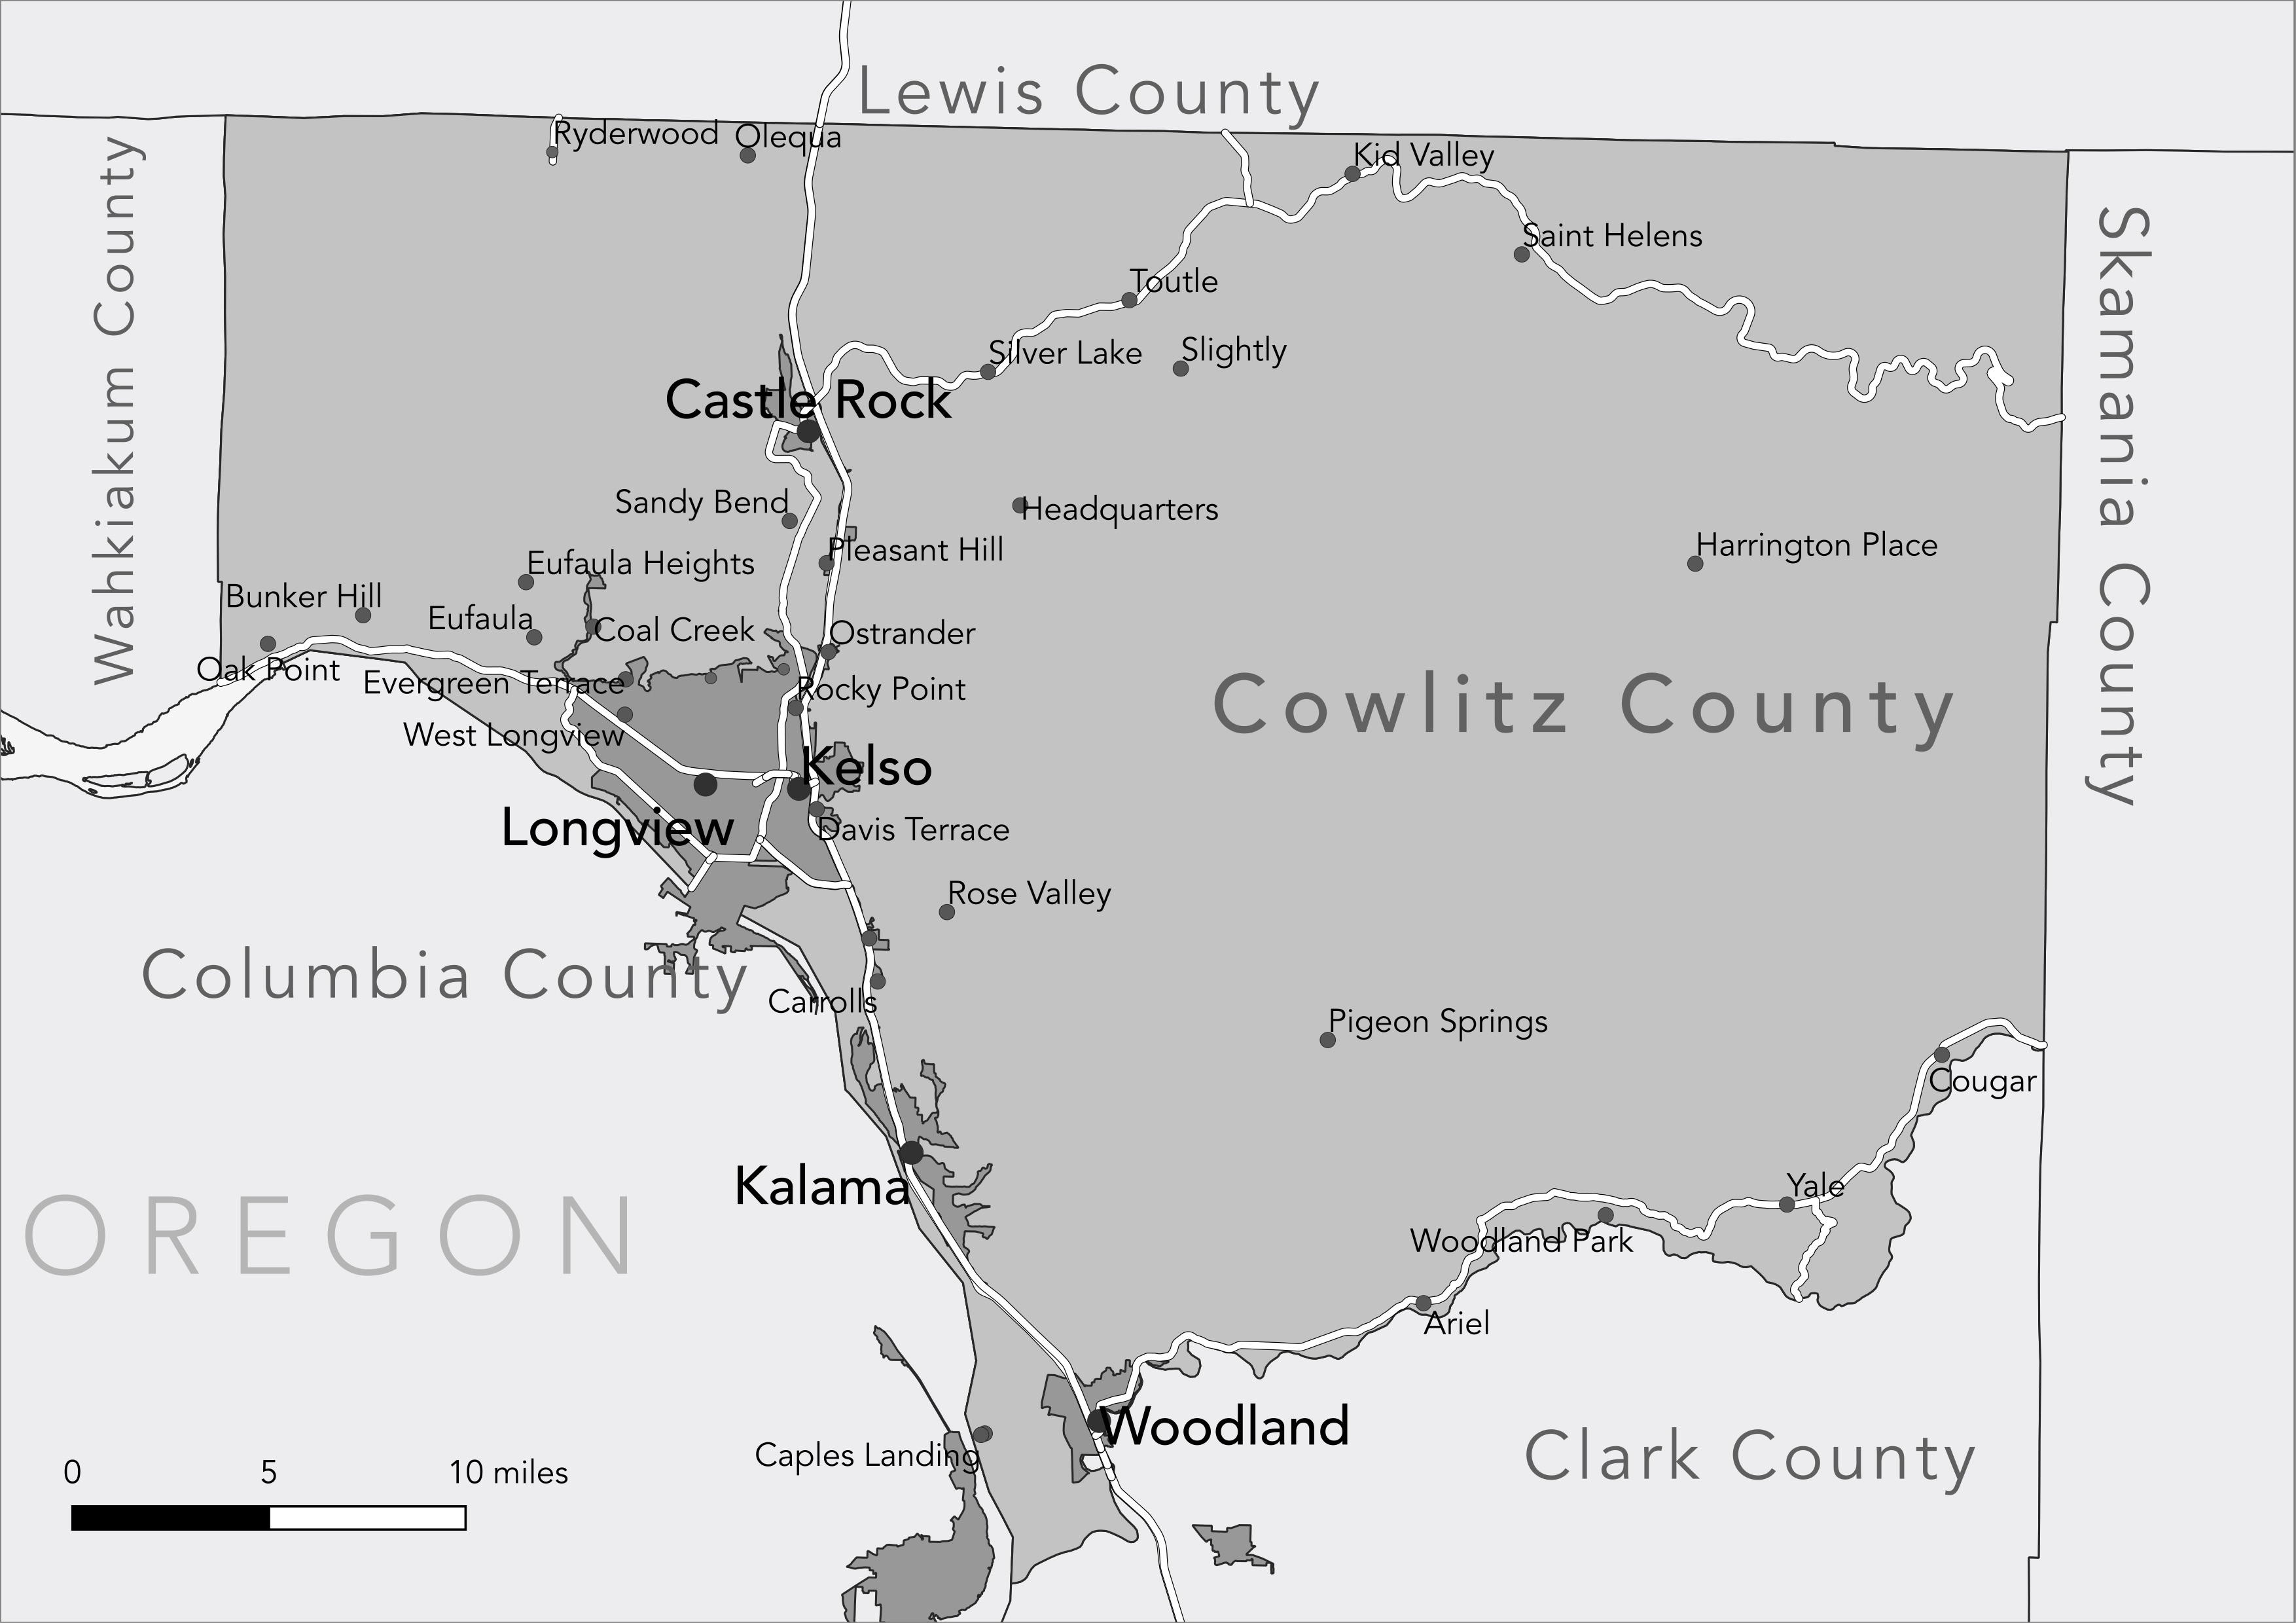
\includegraphics[angle=90, origin=c, width = 5.75in]{Figures/other_figures/Cowlitz_Focus_small.jpg}
    \caption{Cowlitz County, Washington}
    \label{fig:map_of_cowlitz_zoom}
\end{figure*}

Cowlitz County is an area of about 1,139 square miles in southwestern Washington (Figures \ref{fig:map_of_cowlitz_big} and \ref{fig:map_of_cowlitz_zoom}). Its southern border is defined by the Columbia and Lewis Rivers. Its eastern, western, and northern borders are defined by latitude and longitude. It is bordered by Wahkiakum County on the west, Lewis County to the north, Skamania County to the east, and Clark County to the south. Across the Columbia River into Oregon, it borders Columbia County.

Topographically, Cowlitz County is in the Puget Sound-Willamette Depression, meaning it is part of a long stretch of lowland that connects Puget Sound in northwestern Washington with Willamette Valley (as far south as Eugene) in Oregon \citep[2]{barrier_froyalde_1998}. It is located next to the Cascade Range and six major rivers flow from those mountains through Cowlitz County: Columbia, Lewis, Cowlitz, Toutle, Kalama, and Coweeman. On clear days you can see Mount Rainier, Mount St. Helens, Elk Mountain, and Mount Hood. However, such days are rare as rain and cloudy skies are the dominant weather patterns for eight months of the year\footnote{Weather data is taken from WeatherSpark.com.}. The warmest month is August, with an average high temperature of 79\degree F, while the coldest month is January, with an average low temperature of 35\degree F. These moderate climate makes it quite a pleasant place to live. The terrain is rather hilly and large trees (Douglass Fir and many others) cover the area.

The county is home to 102,410 people, putting the population density at 89.9 people per square mile. The five cities in Cowlitz County, with their 2017 estimated populations \citep{census_factfinder} are Longview (36,740), Kelso (11,864), Woodland (5,765), Castle Rock (2,899), and Kalama (2,497). There are an additional 31 unincorporated communities; of them, Carrols, Coal Creek, Oak Point, Ostrander, Rose Valley, Sandy Bend, Stella, and Toutle were mentioned in interviews and have historical significance. Ranier, Oregon shares a border with Cowlitz County is accessible from Longview by bridge. Other notable cities nearby include Portland (50 miles to the south), the Washington suburb of Vancouver, and Seattle (128 miles to the North) and are accessible via Interstate 5 which cuts through the county. Astoria, Oregon is 50 miles to the west and the Pacific coast is just beyond that.

As for the people themselves\footnote{County data is taken from datausa.io.}, residents of Cowlitz County are similar to the rest of Washington in that they are mostly US citizens (97.5\%) and are predominantly white (84.6\%) with Hispanics (8.4\%) forming the largest ethnic minority group. However, the median age of 41.4 is somewhat higher than the rest of the state (36.4) and appears to be increasing. The median household income was \$49,127, which is far lower than the state average of \$67,106. On average, the area is poorer and older than the rest of the state, with the majority of people working in manufacturing as opposed to the rest of the state which has more workers in the restaurant and food industry, construction, and elementary and secondary schools.

\section{The Cowlitz Indian Tribe}

The present-day region of Cowlitz County sits on the ancestral lands of the Cowlitz Indian Tribe.\footnote{According to its contemporary leaders, the official and preferred term for this people is the \textit{Cowlitz Indian Tribe}.} Relatively little is known about this peaceful people, though at one point as many as 50,000 inhabited the region between the Cascades and the mouth of the Columbia River \citep[70]{olson_1948}

Though the Cowlitz were a united group of people, they can still be classified into four primary divisions within the region \citep[8-10]{urrutia_1998}. First, the Lower Cowlitz Indian Tribe formed the largest group and settled on the lower Cowlitz and Kalama rivers. As this was an important trade route between the Columbia River, Puget Sound, and the Klikitats from east of the Cascade Mountains, they were able to garner wealth and establish a lifestyle that was more comfortable than their neighbors. The Upper Cowlitz Indian Tribe primarily lived in small villages and hunting camps along the upper Cowlitz river. Being too far upstream to rely on salmon, they took advantage of the open meadows to grow berries and rode horses to hunt game. Their proximity to Mount Rainier gave them access to trade and with Sahaptin-speaking peoples on the east side of the mountains, and after centuries of intermarriage the Upper Cowlitz spoke both Cowlitz and Sahaptin. The Lower River Cowlitz form the third group, who settled in the meadows of the Lewis River. Like the Upper Cowlitz, they were skilled horsemen. They also had extensive contact with the Klikitats, who often married into and joined Lower River Cowlitz families. The fourth group is sometimes referred to as the Mountain Cowlitz, who lived in the meadows, streams, and prairies east of the Lower Cowlitz River.

These four groups within the Cowlitz illustrate that the key to survival for in this region was adaptation and being intimately connected to nature \citep[10--14]{urrutia_1998}. To thrive in a region that includes rivers, prairies, and mountains, they were expert fisherman, gatherers, and hunters, traveling by canoe, horse, and foot. In addition to Sahaptin spoken by the Upper Cowlitz, the languages of the people were Chinook Jargon and Cowlitz, a Tsamosan language within the Salishan family \citep{lewis_etal_2016_ethnologue}.
However, their numbers declined even before those of European descent began to permanently settle the region. Disease spread throughout the area between 1832 and 1844, significantly reducing their numbers, and sometimes wiping out entire villages \citep[72]{olson_1948}. Today, the Cowlitz language is extinct and what was once a large and thriving people has been reduced to less than 200 individuals \citep{lewis_etal_2016_ethnologue}.

\section{Exploration and discovery}
\label{sec:exploration_discovery}

It is unknown how long the area that is now known as Cowlitz County has been populated. But people of European descent did not see it until October 1792. This is a relatively late date considering that extensive exploration to in Puget Sound to the north and in California to the south that had already occurred.

There were numerous close encounters by previous explorers though \citep[cf.][15-16]{urrutia_1998}. Sir Francis Drake of England, who sailed along the Pacific coast raiding Spanish in 1577, missed the mouth of the Columbia River due to thick fog. The Spanish sailor Bruno Heceta was at the mouth of the Columbia in 1775 according to his latitude, but because his men were so sick with scurvy he did not enter it. Another English seaman, Captain James Cook, saw the Columbia river between 1776 and 1780, but did not enter it because of bad weather and because he was in a hurry to get to the Strait of Juan de Fuca. Britain's John Meares of 1788 was also at the mouth of the Columbia but did not realize that the giant opening was in fact a river. Similarly, Captain George Vancouver noted in 1792 that that the color of the sea resembled a river, but he, too, was convinced that the “bay” was too large to be a river \citep[3]{olson_1948} and sailed northward to the Strait of Juan de Fuca in search of the Northwest Passage—a commercial sea route connecting the Pacific to the Atlantic.

Finally, Robert Gray, a trader and merchant, was the first to enter the Columbia river (\citealt[16]{urrutia_1998}, \citealt[3]{olson_1948}). During his first voyage, he was part of the first American crew to round Cape Horn at the southern tip of South America. Along the Pacific Coast in what is now California, Oregon, and Washington, he explored many rivers, but could not enter one because of the tide. He continued on, sailing to Hawai'i and China before returning back home to Boston via the Cape of Good Hope. On his second voyage, in search of the “Great River of the West,” he went back to explore the river he was not able to enter on his first journey. It was on May 11, 1792 that he and his crew sailed into the Columbia River, becoming the first white explorers to do so, though they traveled no further than 15 miles so they did not see present-day Cowlitz County.

Captain Vancouver, hearing of Captain Gray's entrance and wishing to claim the area for Britain, sent Lieutenant William Broughton and a small crew to explore the Columbia a few months later in October 1792 \citep[16-17]{urrutia_1998}. It was they that were the first white explorers to see the area that is now Cowlitz County, sailing inward as far as what is now Vancouver, Washington. On the way, they met the inhabitants on both sides of the river and designated names for notable features such as Mount Coffin  and Mount St. Helens.

The Lewis and Clark Expedition were also among the early explorers to see Cowlitz County, and were the first to reach the area by land rather than by sea (\citealt[20--23]{urrutia_1998}, \citealt[3--4]{olson_1948}). During November 5--6, 1805, they canoed downstream past what is now Cowlitz County, noting the villages they saw, trading with the inhabitants there, and making observations of wildlife and landmarks, such as Mount Coffin. They technically did not step foot in Cowlitz County though. The team camped on the Washington side of the Columbia river the evening of November 4 before they reached the Lewis River, just south of the present-day county line. The next evening, they camped on the Oregon side across from the Kalama river, and by nightfall November 6th they had just passed what is now the county line again and camped opposite of Wallace Island.

The land around the Columbia river was highly desirable by both the Americans and British and both sides had good arguments for why they should own the land. While Captain Gray was first to enter the Columbia River, Lieutenant Broughton of Britain went further inland. But then Lewis and Clark came to the region from the Rockies, strengthening the idea that the Americans should have the land. However, Welshman David Thompson and his small crew were the first non-indigenous people to sail the Columbia from its source all the way to the Pacific in 1811, meaning the British had a stake at the claim \citep[26]{urrutia_1998}. Both sides knew that the best way to defend a claim was to settle the area.

\section{Settlement and colonization}
\label{sec:settlement_colonization}

Because of the War of 1812, very few settlers crossed the Rockies into the area at that time, so the area of present-day Cowlitz County remained relatively free of newcomers. Part of the reason was also because the Cowlitz Tribe became increasingly hostile towards outsiders because of maltreatment by trappers \citep[31]{urrutia_1998}. This started to change in the 1830s when contention arose between Russia and the newly merged Hudson's Bay Company because of the Canadian-based company's posts in Alaska \citep[27-29]{urrutia_1998}. A deal was made, and the company could lease the land from the Russians in exchange for grains and meat. The question was where the Hudson's Bay Company was supposed to acquire these supplies. The company soon established farms in several areas, including the Cowlitz Valley, using the Cowlitz River as a passageway. Consequently, the first substantial buildings in the area were what the company called the ``Caweeman Post'': two warehouses to store grain and a house for a priest which were built in 1845 about a mile and a half from the mouth of the Cowlitz river.

However, not seeing potential in the Cowlitz or Columbia rivers, the Hudson's Bay Company soon abandoned the Caweeman Post. Before they did though, they hired two men, Joachim Thibeault and Antoine Gobin, to maintain the buildings and cattle that were left there in order to secure the land for Britain. These men joined the few other former workers of the Hudson's Bay Company who had become permanent residents of the area. Adophus Le Lewes of England settled in what is now the city of Woodland at the mouth of the Lewis River, the area where he kept cattle for the Hudson's Bay Company \citep[37]{urrutia_1998}. Quebec-born Simon Plamondon had been living there since 1838: having explored the Cowlitz River and gained favor with a Cowlitz chief, he married into the community and ended up settling in the region with his many children.

While the Hudson's Bay Company had no more interest in the area, living in the West was the dream of many Americans. The east was crowded, dirty, and in an economic depression while the West was nothing but wide open, fertile land. And as of 1850, it was free too: the Donation Land Act was passed, which promised 360 acres a person if they lived on it for four years. Once the forty-ninth parallel was officially established in 1846 as the dividing line between Canada and the United States \citep[9]{olson_1948}, Americans started coming up the Oregon trail and began to settle the area, though it took a few more years for them to come to Cowlitz County because they preferred the more fertile Willamette Valley in Oregon.

From that point, the area very quickly grew from the simple Caweeman Post to several established communities; most of today's municipalities in Cowlitz County can trace their roots to this time. Peter Crawford's claim, which was across the Cowlitz River from where Thibeault and Gobin were living, was made official on December 25, 1847. He called the area Kelso, named after his hometown in Scotland \citep[51]{olson_1948}. At that time, the three of them were the only residents for 40 miles \citep[39]{urrutia_1998}. But by 1849, there were 50 people living around the mouth of the Cowlitz river, so H. D. Huntington established the city of Monticello, named after his hometown in Indiana \citep[12]{olson_1948}. Crawford was a professional surveyor and laid out the main street of Monticello and divided the land into 1-acre lots. Meanwhile, Le Lewes was joined by family members and opened a store on his property. This encouraged others to join and by the 1850s, Woodland was a thriving community complete with a post office, a school, churches, and additional stores \citep[43-45]{urrutia_1998}. By 1850, there were over a thousand people living in the area that would become Cowlitz County \citep[68]{urrutia_1998}.

While these communities were starting to grow, they did so as a part of the Oregon Territory, a massive region created by Congress on August 14, 1848 that included all of present-day Washington, Oregon, and Idaho and parts of Montana and Wyoming \citep[10-11]{olson_1948}. This area was considered too large for a single territory, so in November 1852, delegates met in Monticello and drew up a document proposing the creation of a new territory. Congress approved the bill on February 8, 1853 and gave it the name Washington. One of the first things that was done was to make Olympia the capital and to create several new counties—one of them being Cowlitz. Thus, on April 21, 1854 , Cowlitz County was officially created: the name Cowlitz was a natural choice, and reportedly means either “capturing the medicine spirit” or “peaceful” in the Cowlitz language \citep[11]{olson_1948}.

The lumber industry has always been of primary importance in Cowlitz County \citep[85-88]{urrutia_1998}. Even the earliest settlers built sawmills to make materials for their rafts and houses. George Abernathy, an entrepreneur from New York City, saw the potential of this industry and built a sawmill at Oak Point on western edge of Cowlitz County. Using the power of Mill Creek, his mill had both a vertical and a circular saw and quickly outstripped the production of the two existing mills owned by the Hudson's Bay Company. These saws were quite lucrative for him when he could fill the demand coming from the California Gold Rush starting in 1848 \citep[18-19]{olson_1948}. Inspired by the success of the sawmill at Oak Point, many other sawmills popped up along the various rivers in Cowlitz County.

This demand for lumber only increased when steamboats began to regularly travel along the Columbia River in 1850 \citep[87-91]{urrutia_1998}. These ships burned wood to create steam, so they had to stop regularly at ports to replenish their supply. By 1853, there were five stem engines that regularly traveled from Portland to Astoria, and so communities such as Martin's Bluff and Carrolls profited from these stops by providing shops, hotels, churches, stables, post offices, and of course plenty of wood for sale. Five small communities (Stella, Bunker Hill, Midway, Nisqually, and Oak Point) thrived along a two and a half mile stretch on the west end of Cowlitz County, each with their own shops, hotels, and sawmills or log flumes. Small communities supplied resources to steamboats even on the smaller Cowlitz and Lewis rivers, even though they did not lead to major population centers \citep[99-109]{urrutia_1998}. However, with the exception of Carrolls, each of these communities faded into obscurity by 1900 when steamboats were replaced by trains.

Cowlitz County continued to enjoy a strategic position as trains began to travel the West \citep[92-98]{urrutia_1998}. The Northern Pacific Railroad company surveyed the land and eventually bought land four miles south of Carrolls in 1870 to establish a train station that would be the final stop in a transcontinental railroad. Thus, the city of Kalama was born. The population quickly grew to 3,500 as workers from all over the world built a town around the station, a town that was expected to surpass Portland in size. However, as soon as the route to Tacoma was finished by December 1873 \citep[48]{olson_1948}, Kalama floundered as Northern Pacific moved its headquarters to Tacoma. Regardless, for more than 30 years, Kalama was an important part of Cowlitz County's growth because of its location on key transportation routes. Furthermore, the establishment of trains in the area required the production of innumerable railroad ties, an industry that employed thousands, particularly up the Toutle and Lewis rivers \citep[119]{urrutia_1998}.

Starting in the 1860s, Cowlitz County was also home to a large fishing industry \citep[120-124]{urrutia_1998}. Salmon and smelt were plentiful in the area, and workers in Cowlitz County developed innovative methods of canning, preserving, and packing them to survive shipment overseas. By 1881 there were 35 salmon canaries along the Columbia river \citep[31]{olson_1948}. In the 1890s, hatcheries in Cowlitz County provided millions of Chinook salmon. However, the fishing skidded to a halt when dams were built in 1940, leaving timber as the primary industry in the area.

While logging has always been a key part of Cowlitz County, the magnitude of operations grew to an astronomical scale beginning in the 20th century Frederick Weyerhaeuser of St. Paul, Minnesota bought 900,00 acres from Northern Pacific. Then, when a massive forest fire swept through the region in 1902, it was beneficial to operate more locally, so they set up their base of operations in the small town of Yacolt in Clark County, just to the south of Cowlitz County. For 14 years they harvested the burnt trees and continued their operations until 1924. Meanwhile the mill in Ostrander specialized in cutting very long pieces of lumber (it set the world record of 240 feet in 1905; \citealt[19]{olson_1948}). During the first World War, it ran night and day to keep up with the demand, its wood often serving as posts in freight carriers in the Atlantic \citep[126-129]{urrutia_1998}.





\section{Longview: A planned city}
\label{sec:longview_a_planned_city}

Weyerhaeuser's base of operations in Yacolt was significant, but Cowlitz County was changed forever in 1918 when Robert A. Long and the Long-Bell Lumber Company decided to move from Kansas to the mouth of the Cowlitz River. Long-Bell was a successful timber company in Kansas City, but when its timber began running low, rather than retiring rich, the 68-year-old co-founder and sole-owner of Long-Bell decided to find a more suitable location for the company \citep[1]{mcclelland_1976}. To accompany their purchase of 70,000 acres of forest (containing several billion potential board feet of lumber), they bought an enormous piece of land to establish what would become the largest sawmill on the planet \citep[132-136]{urrutia_1998}. However, to prevent damage from floods, dikes were needed around the valley where the mill was; Mr. Long figured they would just buy out the rest of the valley (13,929 acres, \citealt[18]{mcclelland_1976}) at whatever price the existing settlers and farmers named. And so they did.

With such a large amount of land, Long-Bell was free to build as they suited. They estimated 3–4 thousand workers were required to operate the mill, with another ten thousand required to run a city to support those workers (\citealt[5]{wilma_2017}, \citealt[21]{mcclelland_1976}). Kelso, the newly elected county seat, had a population of 2,500 and was three miles away. Not only was this not a large enough workforce, but few of the residents had cars (and there were no roads leading from Kelso to the new mill site anyway), so an alternative solution was needed. Long-Bell decided the best course of action was to create an entirely new city, one that could support the large population needed to run the mills. Since Long-Bell owned the entire valley, they decided to plan the roads, neighborhoods, and sectors before any construction began. Rather than the untidy effects of an urban sprawl, they \textit{zoned} specific sectors for residential, commercial, and industrial use---a relatively new concept at the time \citep[22]{mcclelland_1976}. Thus, the city of Longview was born in 1923.

Long-Bell had two main goals when starting its city. First, it had to establish the mills. This goal was met less than a year later when they built the two largest sawmills in the world which would soon produce nearly two million board feet of lumber a day. The second priority was to make Longview beautiful. For example, buildings in the main business district could only be built of masonry and had to be at least two stories tall so that they provided grand but harmonious store fronts \citep[27]{mcclelland_1976}. But because the city was zoned, it grew in an unusual patchwork pattern rather than radially from a city center, meaning the roads were paved but largely empty. So Long-Bell built a large six-story hotel, the Monticello Hotel, to attract newcomers to the city. Long himself donated \$1 million to build the library, a high school, and to improve the main church. The company achieved these two goals, and the Longview attracted workers from across the country.

While Longview may have looked impressive, but there were some some aspects of its design that clearly show that the priority was Long-Bell rather than Longview's residents \citep[28--30]{mcclelland_1976}. In the spirit of making the city look nice, many vacant lots were beautifully landscaped; however a playground would not be built for another four years and no sports centers were planned. The waterfront properties were zoned for industrial use because of easy access to the river rather than for housing. (Perhaps their thought was ``Who would want to have a view of the river when our city is so beautiful?'') An imposing train depot was built, yet there was no thought for how people would enter the city by car, other than through Kelso's downtown district. The first residential areas to be developed were close to the mills, but far from the rest of town, forcing the many families without cars to walk the approximately 10 block to shopping centers, schools, and entertainment. All original homes were demolished and rather than naming roads after the original farmers\footnote{In fact, the only nod to any previous people was in the name of the Monticello Hotel. It was named after the city of Monticello which was completely erased once Long-Bell bought out the valley.}---let alone the Cowlitz Indian Tribe---the company's top executives' names were used instead.

In spite of its flaws, a massive influx of workers came to Longview, bringing with them additional manufacturers to Cowlitz County. Weyerhaeuser, with its enormous stockpiles of burnt logs,\footnote{Recall that at this point Weyerhaueser was based in Yacolt to harvest burnt logs from the forest fire in 1902.} constructed three mills adjacent to Long-Bell in 1927 \citep[161-162]{urrutia_1998}. Both of these plants produced an inordinate amount of sawdust and wood chips  which people could burn in their home furnaces. As was typical of that time however, the excess was burned in an enormous wigwam or teepee burner. Wishing to capitalize on the sawdust, Longview Fibre Company was founded in 1927 and began converting all the wood waste from Weyerhaeuser into paper products (\citealt[164--165]{urrutia_1998}, \citealt[11-13]{olson_1948}). A few years later, Reynolds Metal Company was established in 1941 \citep[175]{urrutia_1998}. By 1927, the population of Longview proper had grown to 11,600 \citep[36]{wilma_2017} and together with Long-Bell, these three companies employed several thousand in Cowlitz County.

In terms of place of birth, what was the population of Cowlitz County like at this time? Census records indicate that at least 31,914 individuals were living in Cowlitz County in 1930.\footnote{I obtained these census records using \textit{Family Search} (familysearch.org), a genealogical site owned by the Church of Jesus Christ of Latter-day Saints. I was not able to search by county of residence, so I searched for people living in Longview in 1930, which returned many thousands of records of people living in or near Longview. Data included years, states, and countries of birth and the city and county of residence. Those who lived in another county were excluded. These records are not normally available to download in bulk but I was able to save them in groups of 75 entries at a time. These hundreds of spreadsheets were then combined and analyzed in R.} Figure \ref{fig:census1930} shows that the majority of those living in Cowlitz County who were before 1930 were not from Washington but were in fact from elsewhere in the United States. In fact, even including the many children born after Longview was founded, a full 60\% of 1930 Cowlitz County were nonnatives to Washington.

\begin{figure*}[t!]
    \centering
    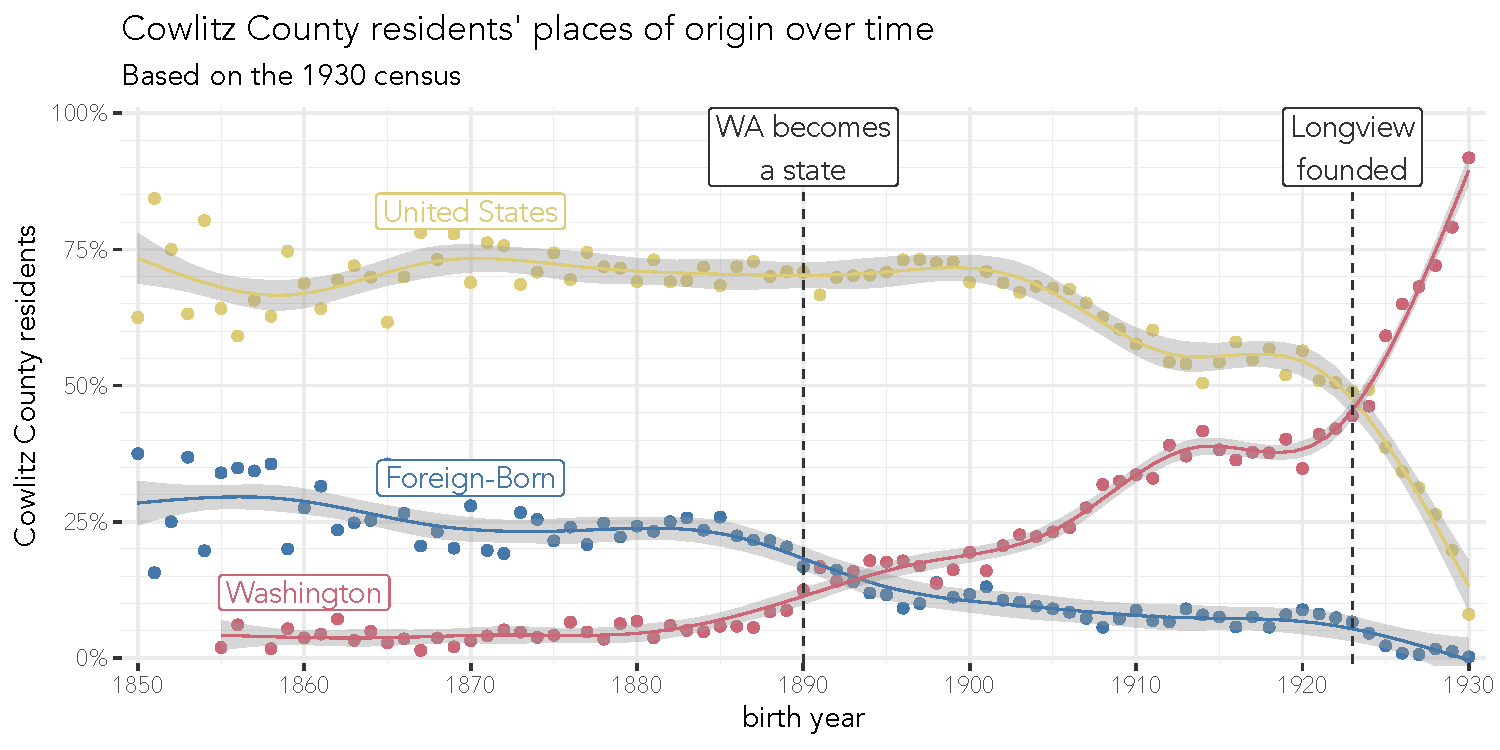
\includegraphics[width = 6.5in]{Figures/other_figures/origin_1930.pdf}
    \caption[Proportion of Cowlitz County residents by year of birth by origin ]{Given the residents living in Cowlitz County in 1930, this chart shows the proportion of origin by year of birth. The 86 octogenarians and five nonagenarians are excluded from this plot since there were so few of them and their averages were so haphazard (the data begins to fan out towards the left of the plot with those born in the 1850s).}
    \label{fig:census1930}
\end{figure*}

A closer look at Figure \ref{fig:census1930} reveals that significant events in the area correlated with demographic shifts. The proportion of foreign-born immigrants in Cowlitz County was actually at its highest all-time high in 1850 and steadily decreased over the decades. There is a small rise in foreign-born immigrants the early 1920s around the time Long-Bell was established, but this fell quickly to near 0\% by 1925. Meanwhile the proportion of people born in Washington (or the area that became Washington) in Cowlitz County has accelerated since the 1850s. They surpassed the foreign-born immigrants around the time Washington became a state and then overtook the non-Washingtonians soon after Longview was founded.

\begin{table}[ht]
    \caption[Number of foreign-born immigrants by country living in Cowlitz County in 1930.]{Number of foreign-born immigrants by country living in Cowlitz County in 1930. The 77 countries that contributed to less than 1\% of the total foreign-born population (36 or fewer people) are excluded. There were 441 people from these excluded countries.}
    \centering
    \liningnums{
        \begin{tabular}{l r r}
            Country     & People & \shortstack{Percent\\(of foreign-born)}\\
            \hline
            Canada      & 1186 & 30.81\%\\
            Finland     &  459 & 11.93\%\\
            Sweden      &  412 & 10.70\%\\
            Norway      &  296 &  7.69\%\\
            England     &  252 &  6.55\%\\
            Germany     &  233 &  6.05\%\\
            Russia      &   94 &  2.44\%\\
            Denmark     &   88 &  2.29\%\\
            Scotland    &   78 &  2.03\%\\
            Switzerland &   59 &  1.53\%\\
            Austria     &   58 &  1.51\%\\
            Ireland     &   57 &  1.48\%\\
            Holland     &   48 &  1.25\%\\
            Poland      &   47 &  1.22\%\\
            Japan       &   41 &  1.07\%
        \end{tabular}
    }
    \label{tab:foreign_born}
\end{table}

\begin{table}[ht]
    \centering
    \liningnums{
        \begin{tabular}{l r r}
            State     & People & \shortstack{Percent\\(of non-Washingtonians)}\\
            \hline
            Oregon       & 3329 & 17.27\%\\
            Minnesota    & 1289 &  6.69\%\\
            Missouri     & 1144 &  5.93\%\\
            Iowa         & 1124 &  5.83\%\\
            Wisconsin    & 1023 &  5.31\%\\
            Kansas       &  904 &  4.69\%\\
            Illinois     &  843 &  4.37\%\\
            Idaho        &  829 &  4.30\%\\
            Montana      &  787 &  4.08\%\\
            Michigan     &  723 &  3.75\%\\
            Nebraska     &  637 &  3.30\%\\
            California   &  545 &  2.83\%\\
            North Dakota &  481 &  2.49\%\\
            Ohio         &  447 &  2.32\%\\
            Indiana      &  445 &  2.31\%\\
            Texas        &  423 &  2.19\%\\
            Colorado     &  391 &  2.03\%
        \end{tabular}
    }
    \caption[Number of non-Washingtonians by state living in Cowlitz County in 1930.]{Number of non-Washingtonians by state living in Cowlitz County in 1930. Only states that contributed to more than 2\% of the total non-Washingtonian population are included here, but all US states were represented in this community. There were 1250 people from the other states.}
    \label{tab:non_washingtonians}
\end{table}

Regarding the non-Washingtonians, the majority come from northern Europe and other northern states. For the foreign-born immigrants, a full 30\% came from Canada, and the majority the rest came from areas such as Scandinavia, Finland, the United Kingdom, and Russia (see Table \ref{tab:foreign_born}). Among the Americans, it comes as no surprise that Oregon is the most represented, given that Cowlitz County is on its border. Many other people came from states now part of the Northern dialect region (Minnesota, Wisconsin, Michigan) or the Midlands (Missouri, Iowa, Kansas, Illinois, etc.). There were very few southerners, New Englanders, and a relatively small proportion of 1930 Cowlitz County came from California.

The Great Depression affected Cowlitz County like the rest of the nation, but despite nearly going bankrupt themselves, Long-Bell, Weyerhaeuser, and Longview Fibre managed to provide many jobs for the community. Part of this had to do with changes in how goods were transported: shippers discovered that it was lighter and cheaper to use corrugated paperboard rather than wooden crates \citep[69]{wilma_2017}, meaning there was an increased demand for paper products. The mills were also flexible in what products they could provide to their clients and producing new items created more jobs. To save on costs though, workers were paid less and could only work every other day, but the unemployment rate was not as high as it was in other parts of the country \citep[167]{urrutia_1998}.

Fear struck the community during the Second World War, but business was still booming. The wartime demand of lumber, paper products, and aluminum kept the manufacturing plants running non-stop, and the debts they incurred during the Great Depression were quickly paid off. Women had always worked in the mills, but around this time they began to take up the manual labor positions formally reserved for men \citep[132]{wilma_2017}. There was also an influx of loggers from California, unemployed due to heavy snow, to help the most pressing need of workers in the forests. More than ever, the mills played an important role for a large proportion of the residents in Cowlitz County.
Into the 1950s, the mills continued to thrive as consumers demanded more paper products. Much of this had to with the new ways that paper was being used. As mentioned previously, shippers switched to paper-based boxes instead of wooden crates, but items such as specialized boxes, such as for clothing or cakes, were being used more and more. Various kinds of paper were manufactured that included items like gift wrap, butchers' paper, and the little sheets of paper between slices of cheese or meat. In addition to paper grocery bags, Longview Fibre was producing special bags made for garments, poultry, nails, popcorn, sugar, and raisins \citep[122-123]{wilma_2017}.

The culture of these companies was to make sure its employees were treated right, though part of this may have been out of obligation and fear of the labor unions. In the early 20th century, unions among loggers in the Pacific Northwest were increasingly popular and grew more powerful, so fair treatment was the best way to avoid confrontation \citep[145]{urrutia_1998}. But the Longview companies went above and beyond what other sawmills did in the Pacific Northwest. Rather than muddy tents for the loggers in the forest, Long-Bell built the small city of Ryderwood, which included family homes, a store, a school, a doctor's office, and a train that took workers to and from Longview. The neighborhoods known today as the Highlands and St. Helen's were filled with modest homes for employees and their families, who could easily afford them with the stable income they brought home. Longview Fibre was concerned about the employees who had to pay the \$1 toll to cross the Columbia River into Longview, so the company used its tug boats to ferry workers over for free \citep[102]{wilma_2017}. If an injury prevented an employee from working, they continued to get their paycheck. This tradition of treating its employees well continued for decades, and as will be shown hereafter, may have set the stage for the sudden language change experienced in the 1970s.

Many of the employees in Longview's mills began work while they were still in high school. They mostly worked in the lowest-wage positions and required little training \citep[133]{wilma_2017}, but they could move their way up after graduation. In fact, Cowlitz County very quickly established the Lower Columbia Junior College in 1934 to provide courses and training in forestry and paper-making \citep[173-174]{urrutia_1998}. Employees' children often worked at the mills as soon as they were old enough to, promoting the idea of it being a family industry.

Working at Longview Fibre always meant there was a possibility of promotion. New hires almost always started at the bottom, but rather than bringing in outside hires to fill middle- and upper-level management, these spots were filled from within the company itself. One worker, Delos Wilma, began his career in 1940 unloading railroad cars and piling wood on steel cars, but retired 42 years later as superintendent of the paper mill \citep[105]{wilma_2017}. Another, Meade Cobb, started part-time while still a high schooler, but ended up as the head of the stereotype department after nearly 40 years \citep[133]{wilma_2017}. This continued until present-day: I was fortunate to interview Rich who tells of his experience in moving up the ladder within the company:
\begin{num_quote}
    "[I] joined with a company- a local company, Longview Fibre Company, as an entry-level designer. So I basically came back to my hometown to start my career. And then went on for twenty-eight years, got a few promotions and… So my job at, uh, Longview Fibre went well and the design and the engineering and I was, uh, at some point the chief engineer and then I- I got a- a step above that.\footnote{Rich is being modest here: he was a former vice president.}" (Rich, 59, M)
    \label{quote:moving_up_coorporate_ladder}
\end{num_quote}
This culture of internal promotion gave workers a sense of belonging and the companies held ceremonies honoring those who worked there for many years. This culture, together with a stable and growing paycheck and a retirement package available to workers as early as 55 years old, was motivation to stay with the company.

During these years of growth in Longview, Kelso was suffering from a bit of an inferiority complex. The 70-year-old city was feeling some resentment from the new city across the river. At first, the rivalry was playful: Kelso girls would boast when they had dates with Longview boys and the football teams in the two cities became arch-rivals. But when increased traffic warranted building another bridge across the Cowlitz River, the antagonism between the two cities escalated \citep[154-155]{urrutia_1998}. Kelso made plans for a bridge connecting south Kelso to downtown Longview, but Longview's plan was to build one nearer to the mouth of the Cowlitz River, connecting Pacific Highway---the only road from Portland to Seattle—to the mills. Longview's plan won out, and in 1926 when the Pioneer Bridge was built, it completely bypassed Kelso. The traffic on Pacific Highway that used to go straight through Kelso's shopping district was diverted into Longview. Consequently, many Kelso businesses moved across the river into Longview, fueling the rivalry between the two cities. Though Kelso and Longview were only divided on a river, they developed “two cultures” \citep[xi]{wilma_2017} as a result of this animosity.

Fortunately, this hostility appears to have calmed down to merely being playful again. Cooperation finally led to the formation of the Greater Longview-Kelso Community Council and they built the Peter Crawford-Cowlitz Way Bridge in 1952. Megan \ref{quote:kelso_depends_on_longview} realizes that both cities exist because of the other:
\begin{num_quote}
    Kelso would have shriveled up and died without the airport and the train station and also the interstate… Even with that it would've just been a teeny tiny town that nobody would've ever heard of and didn't have anything. Except Robert A. Long came and made Longview a spot on the map… So, without Robert A. Long and Longview, Kelso would have died out. So, since I understand that, I'm okay now. But yeah in high school it was totally- I had my church friends who were from Longview, so it didn't really matter as much to me. But it was still like a- every time Kelso or one of the Longview schools play against each other I expect Kelso to beat Longview and I'm thoroughly disappointed if that doesn't happen. (Megan, F, b. 1992)
    \label{quote:kelso_depends_on_longview}
\end{num_quote}
Rob \ref{quote:not_gonna_happen} also mentions the rivalry between Kelso and Longview and explains that while it has calmed down, it still exists somewhat in the community.
\begin{num_quote}
\textit{Have you noticed any animosity between people from Longview and people from Kelso?}

Oh, from the day I was born, yeah. Just the city rivalry type thing. And the football teams would play each other every year the basketball teams and, y'know, it- it was just one of those things and it- it was a big deal for the people of the area to be combative somewhat. And sometimes it got out of hand, sometimes it didn't. But the- that's why the two towns could never combine. Every time you talk about combining, uh, no no, uh, too many people would have hard feelings and say, ``Not gonna happen.'' Never has. (Rob, M, b. 1942)
\label{quote:not_gonna_happen}
\end{num_quote}
This rivalry does not appear to have manifested itself linguistically in the community, but it helps describe the culture one might find among the long-term residents in Cowlitz County.






\section{The rise and fall of the mills}
\label{sec:rise_and_fall}

As described in the previous section, the mills in Cowlitz County were an integral part of the community. They were flexible enough to take advantage of changes in the economy and could recover from devastating blows like the Great Depression or the Columbus Day Storm.\footnote{Columbus Day Storm was October 12, 1962. In reality it was more than a storm and was an ``extra-tropical cyclone originating in the North Pacific'' \citep[185]{wilma_2017}. Winds reached up to 80 miles per hour, much of Cowlitz County was without power for a week, and forty-six people died with hundreds other injured. In addition to the devastating property damage within the county, the storm damaged hundreds of thousands of acres of forest owned by Cowlitz County companies. Fortunately, these fallen trees could be salvaged over the next couple of years, and the products that could be made from them were highly desirable in Japan at the time.} And their significance was not limited to their local communities: Long-Bell, Weyerhaeuser, and Longview Fibre were known regionally, nationally, and across the world. However, in as early as the 1960s, some seeds were being planted that would eventually bring the businesses down, effectively transforming the culture of Cowlitz County from a milling community to something else entirely.

Even though Longview was created because of Long-Bell, their importance on the community decreased over time. Technology advanced, and as cars became more affordable, people could live further from Longview. This made the community less centralized and it diminished the importance of the mills as the primary cultural hub of town. Meanwhile, the demand for paper was as high as ever, and larger paper companies gobbled up smaller ones at this time. For example, Weyerhaeuser expanded to the pulp and paper industry in 1964. Long-Bell was not so well off, and when they merged with International Paper in 1965, they demolished their two massive sawmills to accommodate the new machinery. As a testament to the decentralization of the mills in Longview, one only need to compare the city's reactions to Long-Bell's first and last days. On July 24, 1924 when the first log was loaded onto the headrig, the entire city celebrated with a 4-day pageant that included parades, a rodeo, and a circus \citep[144]{urrutia_1998}. Forty years and 8.7 billion board feet later when the last log went though, Urrutia explains that ``[t]he city of Longview, completely cut off from the apron strings of the founding company, by that time had enjoyed such independence from being thought of as a company town that it scarcely took note of the demise of its parent'' \citeyear[188]{urrutia_1998}. The mills were still among the largest employers in the county, but they were seen simply as a place of work rather than part of the town's identity.

Early 20th century labor unions, as described in the previous section, made sure that mill workers were treated well. However, starting in 1967, these unions—more organized and larger than before—began negotiations with the employers after several years of intermittent strikes \citep[196-198]{wilma_2017}. While this was going on, inflation was increasing faster than ever in the early 1970s, and this of course had an effect at in every part of the business from buying materials, selling costs, and salaries. Employees were demanding raises as high as 10\% a year, and companies like Longview Fibre could not keep up. There was an energy crisis in 1973 and a slump in the number of homes being constructed in 1974 which reduced the amount of timber that could be sold \citep[218]{wilma_2017}. New environmental laws around this time also cut into companies' profits as they had to spend millions on treatment systems.

The pivotal year was 1977. The mills were struggling already after several years of lower production due to strikes and wage increases. But when the price of oil went up, meaning shipments to Japan were costing more and more, companies could not keep up with wage increases. Employees at mills all across the Pacific Northwest were going on strikes and approximately ten thousand workers walked. In Longview, there was hostility towards salaried employees and executives who did continue to work, and while most of it was nonviolent, there were minor incidents such as slashing car tires \citep[200-202]{wilma_2017}. These strikes continued for several years.

As a result of this and other outside forces, the 1980s was a rough time for the timber industry in Cowlitz County. The number of employees working involved in the mills and other timber-related production peaked at 12,210 in 1977 in Cowlitz County and steadily declined since then. Though the companies were still mostly profitable, their impact on the community and the number of jobs they provided was decreasing every year. Longview Fibre went into debt for the first time—by \$113.9 million—in 1981. This marked a clear beginning to its downfall that would eventually lead to their being bought out in 2007. The companies were still loyal to their employees as much as they could be, continuing to pay dividends to stockholders and keeping as many jobs as possible. The state of Washington as a whole was hit hard by the national recession in the early 1980s, but unemployment in Cowlitz County soared, far above even the state average, to 17.5\% at that time. The eruption of Mount St. Helens in 1980 may not have had a significant long-term effect, but it exacerbated the increasing problems in the area at least for a short while.\footnote{Mount St. Helens, a volcano just 36 miles due east of Longview as the crow files, erupted in May of 1980. The direction of the explosion was northward and the winds blew east, so Longview only saw a few centimeters of ash. However, closer to the volcano, this ash made logging in the woods far more difficult as it quickly wore down the chainsaws. Not only were thousands of acres of timber destroyed, but the Cowlitz River flooded with mud, causing evacuations in some areas. It was also full from shore-to-shore of downed timber, causing destruction of property as it hurled these giant trees along at 60mph. In my interviews, I was fortunate to hear many first-hand stories of life in the months after Mount St. Helens blew.} The price of raw goods skyrocketed, outpacing inflation, meaning companies made less and less profit \citep[268]{wilma_2017}. Many companies were moving manufacturing plants offshore, further reducing the number of jobs available to local residents.

This sudden change in town was observed by its residents. Carol \ref{quote:mt_st_helens}, who had several family members lose their jobs in the early 1980s, says this about the changing community:
\begin{num_quote}
    "There were a lot of people that worked in the woods, and if they didn't work in the woods they were like support system, like office people\ldots A lot of people lost their jobs and a lot of people moved. A lot of people just got out of here. And so you take that kind of income from these people out in the woods—and they made really good money considering, y'know—okay, so what does that do to the rest of your economy? They're no longer buying as much gas. They can't afford to go out and go to the movies and eat out and groceries… So yeah. It hit us especially hard." (Carol, F, 57).
\label{quote:mt_st_helens}
\end{num_quote}
Similarly, Teresa points out the increased difficulty in finding jobs affected the culture of the area:
\begin{num_quote}
    ``[In the 1960s and 1970s,] it probably felt more rural or more isolated because people didn't really move away that much then. You know what I'm saying, people were just here, they expected- a lot of guys expected just to go get jobs in the mills and that started changing of course in the eighties. So um so my generation's probably the last generation that got grandfathered into their jobs. So, so that has changed and also our community has changed since that time. Yeah, it's cuz those jobs aren't available anymore, so.'' (Teresa, F, b. 1956)
\label{quote:changed_culture}
\end{num_quote}
Throughout most of the 1980s, the population of Cowlitz County increased because births outnumbered deaths, but more people left than there were immigrants into town. It took until 1987 for the unemployment rate in Cowlitz County to fall below 10\% again.

People also commented on changes within the companies. The mills used to be considered family companies and places where it was easy to get jobs, even while still in high school. But Bruce \ref{quote:easy_To_find_work}, who comes from a family of loggers, noted the difficulty that people have in getting jobs recently:
\begin{num_quote}
    "Back then, everybody… could find work. Y'know somebody had a job say, ‘Hey there's an opening. Come in.' And it's who you know. And go right to work. Like my dad, y'know, you just say, ‘I got a son.' Well they just hired him and went to work. Now, I hear, they don't have the degree. They don't have the knowledge to run the paper machines. So, I hear on the radio they're always advertising, ‘Okay there's a special guy to run the machinery. We don't have anybody [who's] qualified to run these new fancy machines.' So now you have to hire these college kids… Yeah so things change a lot to technology. So it's not like you can't just go in there and work so it's… everything is advanced now." (Bruce, 58, M)
\label{quote:easy_To_find_work}
\end{num_quote}
Historically, people started with the unskilled jobs, there were always opportunities to move up, and middle- and upper-management positions were always filled from within. The qualification to work in management positions was simply experience within the company rather than a college degree. But Harold \ref{quote:family_company}, who worked at the mills his whole life, shares this insider's perspective about the effects of increased automation and the use of technology:
\begin{num_quote}
    "At that time [in the 1970s], it was a family company. Everybody wanted their sons to work there or their daughters to work there. And then it slowly started changing… and it started getting away from a family wage job. It started getting away from guys that knew their profession working up through the ranks so your boss knew the job. By the time I retired forty years later, all the bosses were college graduates with an engineering degree that they thought automatically could tell the guy with forty years' experience how to do the job." (Herold, M, 1949)
\label{quote:family_company}
\end{num_quote}
Putting it more succinctly, Ed \ref{quote:down_the_tube} simply says:
\begin{num_quote}
I grew up in good times. The sixties was a good era, the seventies was good, eighties. And then it started going down the tube. (Ed, M, b. 1949)
\label{quote:down_the_tube}
\end{num_quote}
The topic of the changing economy in the 1970s and 1980s was not mentioned by all of the interviewees and it was only during the course of data collection that I became aware of it and its impact on the community. But the fact that several of these people talked about it unprompted supports the idea that it was a significant change in the community. As a point of comparison, there were only two passing references to the recession of the late 2000s in all of the 54 interviews.

These changes had a lasting effect on the community. At its peak, manufacturing jobs accounted for 45\% of the total income in the county. Twenty years later in 1996, this dropped to 27\% and in 2015 it was approximately one-sixth of the total income. Not only are fewer people working at the mills but their salaries are lower, relative to the rest of the country. In fact, the inflation-adjusted earnings per capita peaked in 1977 at \$19,352 before falling drastically to less than \$15,926 in 1985. It took Cowlitz County twenty years to return to the level it was at in the 1970s.

Into the 2000s, Longview Fibre, one of the few successful mills in the area in the 1980s, had to reduce the variety of products it could provide to its customers. Just as new products created new jobs in its early days, cutting products meant layoffs and, consequently, less revenue coming into the community. It also had to reduce the dividends its stockholders had come to rely on. Eventually, it was bought out and fell into the hands of Kapstone in 2007. However, unlike the machines belonging to other former companies in county, Fibre's mills continue to operate, meaning there are still at least some timber-related jobs in the area.





\section{Cowlitz County today}

Summarizing its history, it is clear that Cowlitz County has had its ups and downs. Its strategic position on a transportation route allowed it to flourish during the 19th century (just as the Cowlitz Indian Tribe had before European explorers). When giant milling operations came to the area in the 1920s, the population exploded, creating the city of Longview and a thriving community where high-paying jobs were easy to acquire. But, after 50 years of plenty, these companies could not keep up with the sudden and simultaneous onslaught of new economic pressures. The industry buckled, sending the community into a 20-year recession.

Cowlitz County has never returned to the thriving community it once was. \citet{bailey_2016} reports that over the last few decades, the unemployment rate has consistently been higher than the national average. During the recession in the late 2000s, it was at one point as high as 15\% and it took until 2017 to bring it back to pre-2008 levels. The inflation-adjusted earnings per capita peaked in 1977 at \$19,352, and after falling to \$15,926 in 1985 it would take until 2000 to recover. The population was relatively stagnant through the 1980s, and Longview has never reached the goal of 50,000 that it was originally designed for.

With this background in mind, I will now present the methods and results of this study in the following chapters. The major events in the history of Cowlitz County, namely the establishment of Long-Bell in 1923 and then the subsequent decentralization of the timber industry in the 1970s and 1980s caused large demographic and attitudinal shifts in the community, shifts that correlated with changes in vowel pronunciation. Therefore, in addition to pressures from neighboring regions, I show that these local changes are linked with the Elsewhere Shift in Cowlitz County.
